% ==============================================================================
% LAB 119
% UNDERSÖKNING AV RC-KRETS
% ------------------------
%
% Author:
% Jonas Sjöberg     <tel12jsg@student.hig.se>
%
% License:
% Creative Commons Attribution-NonCommercial-ShareAlike 4.0 International
% See LICENSE.md for full licensing information.
% ==============================================================================

\section{Beräkning av stegsvaret}\label{step}
% ------------------------------------------------------------------------------

% TODO: Graf för typiskt exponentiellt stegsvar.

Stegsvaret mäts genom att kretsen matas med en fyrkantsvåg med en periodtid som
är tillräckligt lång för att utsignalen ($V_{out}$ i Figur~\ref{fig:rc-schema})
ska hinna uppnå sitt slutvärde för varje halvperiod.

Kretsens tidskonstant beräknas med sambandet i ekv.~\eqref{eq:timeconstant-1}.
Beräkning med ideala komponentvärden enligt ekv.~\eqref{eq:timeconstant-2} samt
faktiska uppmätta komponentvärden i ekv.~\eqref{eq:timeconstant-3}.

\begin{equation}\label{eq:timeconstant-1}
  \begin{split}
    $\tau &= R \times C                                 \\
  \end{split}
\end{equation}

\begin{equation}\label{eq:timeconstant-2}
  \begin{split}
    $\tau &= \SI{1}{\kohm} \times \SI{100}{\nano\farad} \\
          &= \num{1e3} \times \num{100e-9}              \\
          &= \num{1e-4}                                 \\
    $\tau &= \SI{100}{\micro\second}                    \\
  \end{split}
\end{equation}

\begin{equation}\label{eq:timeconstant-3}
  \begin{split}
    $\tau &= \SI{995}{\ohm} \times \SI{110.5}{\nano\farad} \\
          &= \num{995} \times \num{110.5e-9}               \\
          &= \num{1099475e-10}                             \\
    $\tau &\approx \SI{109.9}{\micro\second}                \\
  \end{split}
\end{equation}


\section{Uppmätning av stegsvaret}\label{step}
% ------------------------------------------------------------------------------
Signalgeneratorns trigggerutgång används för att generera en fyrkantsvåg med en
amplitud på \SI{5}{\volt} och en signalfrekvens på \SI{821.6}{\Hz}.


\subsection{Falltid}
% ------------------------------------------------------------------------------
\par Vi söker den tid det tar för signalan att gå från \SI{0}{\volt} till $0.63
\times \SI{5}{\volt} \approx \SI{3.15}{\volt}$. Det ryms uppskattningsvis 1.8
--- 2 divisioner under den aktuella perioden, med tidbasen inställd på
\SI{0.1}{\ms} ger det en falltid enligt ekv.~\eqref{eq:falltime}.

Mätningen av falltide visas i Figur~\ref{fig:fall-foto}.

\begin{equation}\label{eq:falltime}
  \begin{split}
    T_{fall} &= 3 \times \text{div} \times \frac{\SI{0.1}{\mS}}{\text{div}} \\
    T_{fall} &\approx \SIrange{180}{200}}{\ms}  \\
  \end{split}
\end{equation}

\begin{figure}
  \centering
  \includegraphics[width=\linewidth]{img/step_fall.jpg}
  \caption[] {Mätning av falltid.}
  \label{fig:fall-foto}
\end{figure}


\subsection{Stigtid}
% ------------------------------------------------------------------------------
Då signalgeneratorn inte har särskilt god drivförmåga och sannolikt en
osymmetrisk utgångsimpedans, mäts även stigtiden som sedan beräknas enligt
ekv.~\eqref{eq:risetime}.

Mätningen av falltide visas i Figur~\ref{fig:stig-foto}.

\begin{equation}\label{eq:risetime}
  \begin{split}
    T_{stig} &= \dfrac{\SI{50}{\micro\second}}{\text{div}} \times 3 \times div \\
    T_{stig} &\approx \SI{150}{\micro\second} \\
    %T_{rise} &\approx \numrange{180}{200} \si{\micro\second} \\
  \end{split}
\end{equation}

\begin{figure}
  \centering
  \includegraphics[width=\linewidth]{img/step_stig.jpg}
  \caption[] {Mätning av stigtid.}
  \label{fig:stig-foto}
\end{figure}


\subsection{Mätresultat}\label{}
% ------------------------------------------------------------------------------
% TODO: Mätresultat ..


\subsection{Simulering}\label{}
% ------------------------------------------------------------------------------
Kretsen simuleras i \texttt{Qucs} enligt Figur~\ref{fig:step-sim-step} och
Figur~\ref{fig:step-sim-param}.

Figur~\ref{fig:step-sim-step} visar det enkla fallet. En fyrkantsvåg används
för att illustrera hur kretsen svarar mot plötsliga förändringar. Grafen visar
spänningen vid punkten \texttt{Vout} som en funktion av tid.

Figur~\ref{fig:step-sim-param} visar samma skeende då värdet av $C_1$ sätts
till några av vanligt förekommande värden (standardiserade i \texttt{IEC
60063:1963}) genom en ''\emph{parameter sweep}``.  \par
Värden av $C_1$: \SI{10}{\nano\farad},  \SI{100}{\nano\farad},
                 \SI{220}{\nano\farad}, \SI{470}{\nano\farad},
                 \SI{1}{\micro\farad},  \SI{2.2}{\micro\farad}
             och \SI{4.7}{\micro\farad}.


\begin{figure}[ht]\label{fig:step-sim-step}
  \centering
  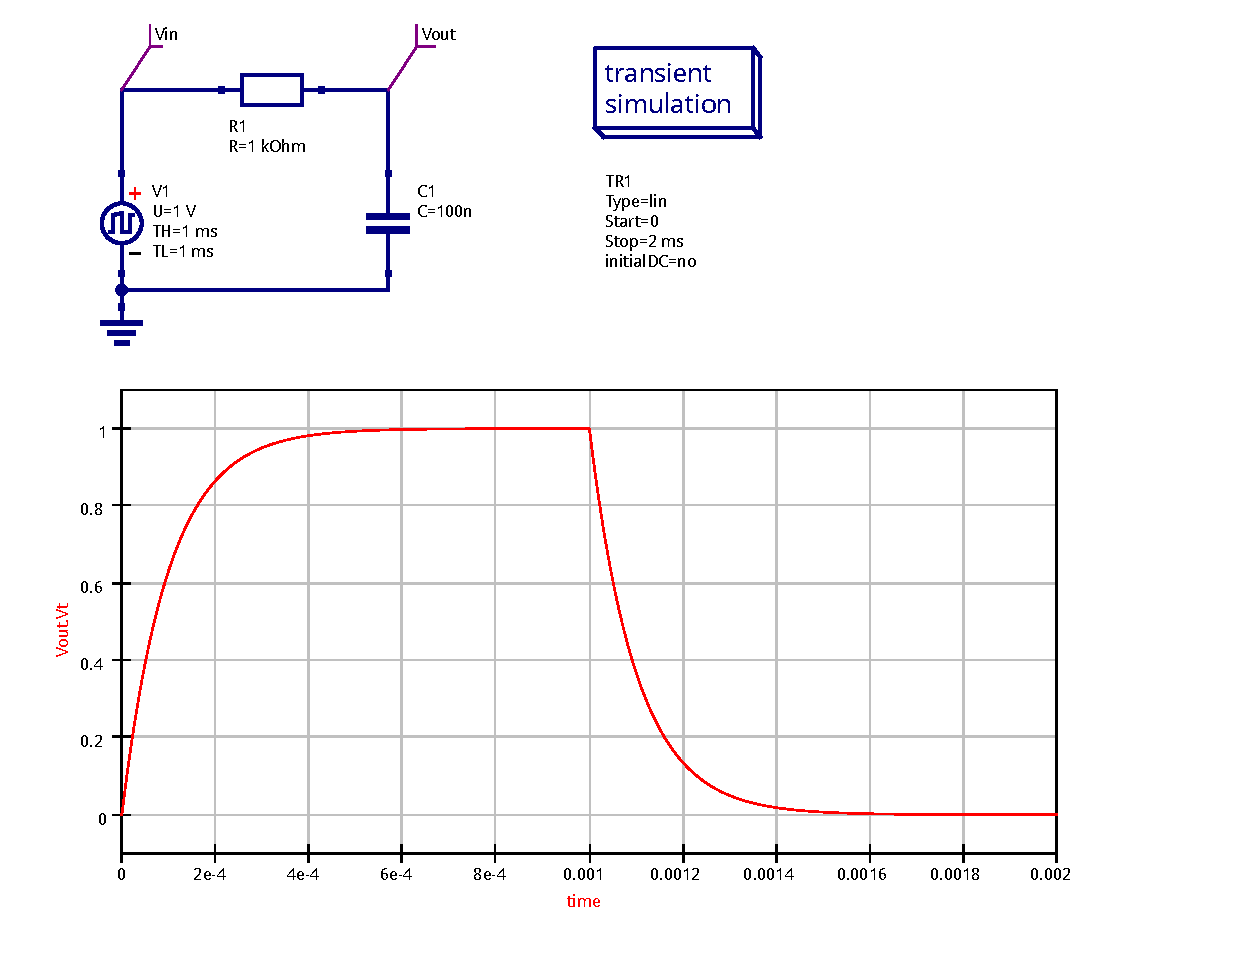
\includegraphics[width=\linewidth]{sim/ee466_lab-4_prj/uppgift-2_step}
  \caption[] {Simulering av kretsens stegsvar.}
\end{figure}

\begin{figure}[ht]\label{fig:step-sim-param}
  \centering
  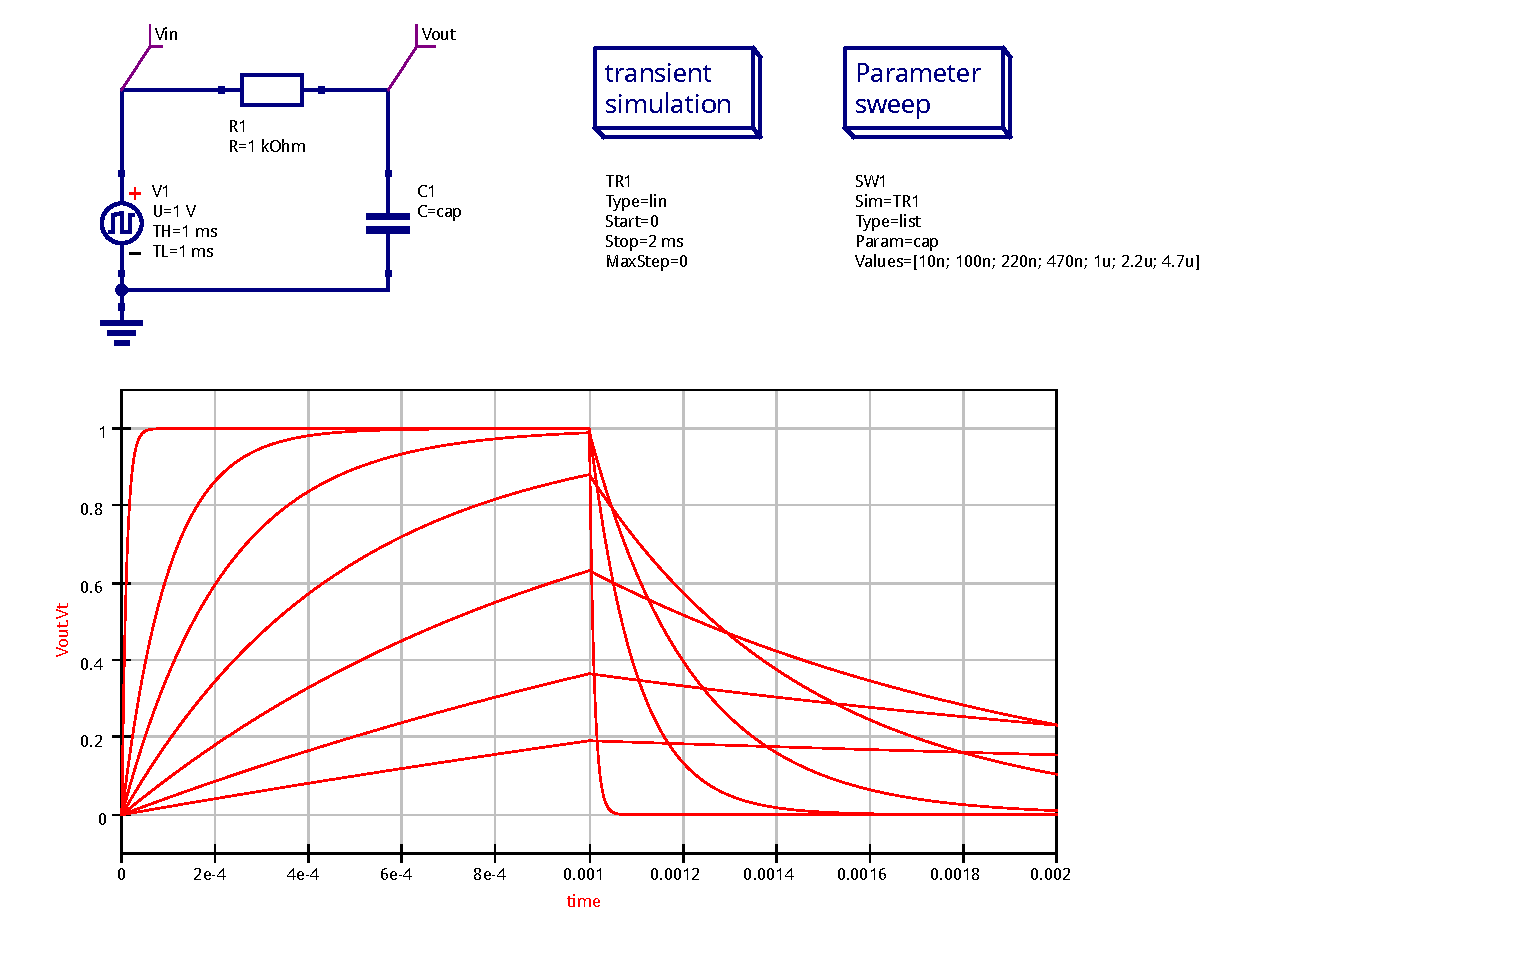
\includegraphics[width=\linewidth]{sim/ee466_lab-4_prj/uppgift-2_param}
  \caption[] {Simulering av kretsens stegsvar för olika värden av $C_1$.}
\end{figure}


\subsection{Kommentar}\label{}
% ------------------------------------------------------------------------------
% TODO: Hur stämmer deta uppmätta värdet av tidskonstanten med det beräknade
%       värdet och med det som erhölls ur Bode-diagrammet?

